\documentclass{../../physics_notes}

\title{Complex Analysis}
\author{St Aidan's Physics Society}
\date{\today}

\usetikzlibrary{decorations}
\usetikzlibrary{decorations.pathmorphing}

\begin{document}

\maketitle

\section*{Introduction}

These notes are based on the Complex Analysis course delivered in Michaelmas 2019, by Prof Ruth Gregory. 

There are also frequent references, both explicit and otherwise, made to the book \emph{Mathematical Methods for Physics and Engineering} by K. F. Riley, M. P. Hobson, and S. J. Bence. Relevant chapters of the book are highlighted using coloured square brackets, e.g. \book{24.5}.

Contributors: Ben Amies-King

\section{The $\mathbb{C}$ plane}
\subsection{Complex numbers}

A simple motivation for studying complex numbers can be gained by considering the roots of a quadratic of negative determinant, such as:

\begin{equation}\label{eq:complex_quad}
x^2 -2x + 2 = 0
\end{equation}

which has roots:

\begin{align}
x &= \frac{2 \pm 2\sqrt{-1}}{2} \nonumber \\
&= 1 \pm i \nonumber
\end{align}

where we denote $\sqrt{-1}$ with $i$. This is the conventional representation of a complex number:

\begin{equation}
z = x + iy = \Re\{z\} + i\Im\{z\}
\end{equation}

We can also express $z$ as coordinates on an Argand diagram, $z = (x,y)$. The roots of equation \ref{eq:complex_quad} are shown in this form in figure \ref{fig:argand_quad}.

\begin{figure}\label{fig:argand_quad}
\centering
\begin{tikzpicture}
    \begin{scope}[thick,font=\scriptsize]
    % Axes:
    % Are simply drawn using line with the `->` option to make them arrows:
    % The main labels of the axes can be places using `node`s:
    \draw [->] (-2,0) -- (2,0) node [above]  {$\Re\{z\}$};
    \draw [->] (0,-2) -- (0,2) node [left] {$\Im\{z\}$};

    % Points
    \draw (1,1) circle[radius=1pt];
    \draw (1,-1) circle[radius=1pt];

    % Axes labels:
    \draw (1,-3pt) -- (1,3pt)   node [above] {$1$};
    \draw (-1,-3pt) -- (-1,3pt) node [above] {$-1$};
    \draw (-3pt,1) -- (3pt,1)   node [right] {$i$};
    \draw (-3pt,-1) -- (3pt,-1) node [right] {$-i$};

    \end{scope}
\end{tikzpicture}
\caption{The complex numbers $z = 1 \pm i$ represented on an Argand diagram. }
\end{figure}

We define the modulus and argument of the complex number $z = x + iy$:

\begin{align*}
|z| &= \sqrt{x^2 + y^2} \\ \\
arg\{z\} &= \tan^{-1}{\frac{y}{x}}
\end{align*}

This leads into an alternative expression of complex numbers known as the polar representation:

\begin{align*}
z = x + iy \longrightarrow z = r e^{i\theta}; \; r  = |z|, \, \theta = arg\{z\}
\end{align*}

We must also define the complex conjugate $z^{\star}$ of $z$, given by:

\[ z^{\star} = x - iy = \Re\{z\} - i\Im\{z\} \]

which implies:

\begin{align*} 
\Re\{z^\star\} &= \Re\{z\}\\ 
\Im\{z^\star\} &= -\Im\{z\} \\ 
|z^\star| &= |z| \\ 
arg\{z^\star\} &= -arg\{z\} 
\end{align*}

We can then deduce:

\begin{equation}
\Re\{z\} = \frac{z + z^\star}{2} 
\end{equation}
\begin{equation}
\Im\{z\} = \frac{z - z^\star}{2}
\end{equation}

The behaviour of complex numbers under simple manipulations (addition, multiplication, exponentiation etc.) can be determined from the polar expression, and so we won't go into it here. 

\subsection{Complex functions}

We can define a complex function $f$:

\begin{align*}
f: \; \mathbb{C} &\rightarrow \mathbb{C} \\
z &\rightarrow f(z) = u(x, y) + iv(x, y)
\end{align*}

where $u, v$ are real functions of real variables $x, y$. For example:

\begin{enumerate}
\item{Polynomials, $f(z) = z^2$ \begin{align*} f(x + iy) &= (x + iy)^2 \\ &= x^2 + 2ixy - y^2 \\ &= x^2 - y^2 + i2xy\end{align*} \\ So $u(x, y) = x^2 - y^2, \, v(x, y) = 2xy$}
\item{Fractional exponents, $f(z) = \sqrt{z}$ \begin{align*} f(re^{i\theta}) &= \sqrt{re^{i\theta}} \\ &= \sqrt{r} e^{\frac{i\theta}{2}}\end{align*} \\ So $u = \sqrt{r}\cos{\frac{\theta}{2}}, \, v = \sqrt{r}\sin{\frac{\theta}{2}}$}
\end{enumerate}

We haven't explicitly specified a range for $\theta$, however it is clear that we will need at least $\theta \in \left[0, 2\pi\right]$ in order to define contours over the whole complex plane. We must then consider multivaluedness of certain functions, as it this will otherwise pose problems when we come to consider concepts such as integration. 

From above, when $f(z) = \sqrt{z}$:

\begin{equation*}
f(re^{i\theta}) = \sqrt{r} e^{\frac{i\theta}{2}}
\end{equation*}

We can clearly see that adding $2\pi n$ to the argument of a complex number $z = re^{i\theta}$ returns the same complex number:

\[re^{i(\theta + 2\pi n)} = re^{i\theta}\cdot e^{i 2\pi n} = re^{i\theta}\cdot 1^n = re^{i\theta} \]

However, putting $re^{i(\theta + 2\pi n)}$ into $f(z) = \sqrt{z}$ produces a concering result:

\begin{align*}
f(re^{i(\theta + 2\pi n)}) &= \sqrt{r} e^{\frac{i(\theta + 2\pi n)}{2}} \\
&= \sqrt{r} e^{\frac{i\theta}{2}}\cdot e^{i \pi n} \\
&= \sqrt{r} e^{\frac{i\theta}{2}}\cdot (-1)^n 
\end{align*}

So for odd $n$, we have that $f(z) = -\sqrt{z}$. Traversing any closed contour results in a change of sign of $f(z)$: it switches to a different branch when crossing the real axis. Now consider $f(z) = \ln{z}$:

\begin{align*}
f(re^{i(\theta + 2\pi n)}) &= \ln{re^{i\theta + 2\pi n}} \\
&= \ln{r} + \ln{e^{i\theta}} + \ln{e^{i 2\pi n}} \\
&= \ln{r} + i(\theta + 2\pi n)
\end{align*}

Hence every full contour traversal, $f(z)$ changes value and never returns to its original. This multivaluedness defies a key property called analyticity, which we will cover later, so we need a solution to force functions to become single valued. 

\subsubsection*{Branch points and branch cuts \book{24.5}}

In the case of $f(z = \sqrt{z}$, we can see that any contour that traverses the real axis only once must contain the origin (and this is unique the origin in this case), and so  we call the origin a \emph{branch point}. We construct a corresponding \emph{branch cut} from the origin to infinity (in any direction, however generally along the real axis). This branch cut is an impassable barrier from the perspective of any contour, and so we are forcing $f(z)$ to be single valued. 

\begin{figure}
\centering
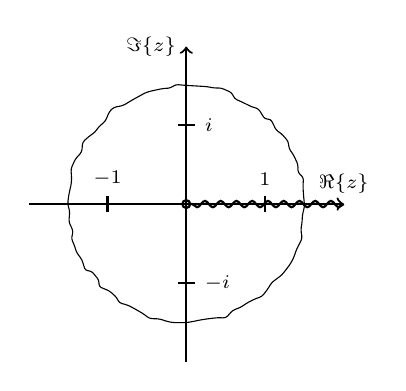
\begin{tikzpicture}
\begin{scope}[thick,font=\scriptsize]
    % Axes:
    % Are simply drawn using line with the `->` option to make them arrows:
    % The main labels of the axes can be places using `node`s:
    \draw [->] (-2,0) -- (2,0) node [above]  {$\Re\{z\}$};
    \draw [->] (0,-2) -- (0,2) node [left] {$\Im\{z\}$};

    % Points
    \draw [decorate,decoration={snake,amplitude=.4mm,segment length=2mm}] (2,0) -- (0,0) node [draw=black, circle, fill=none, inner sep=1pt, pos=1, label] {};


    % Axes labels:
    \draw (1,-3pt) -- (1,3pt)   node [above] {$1$};
    \draw (-1,-3pt) -- (-1,3pt) node [above] {$-1$};
    \draw (-3pt,1) -- (3pt,1)   node [right] {$i$};
    \draw (-3pt,-1) -- (3pt,-1) node [right] {$-i$};
    \end{scope}
	\begin{scope}[decoration={random steps,segment length=3pt,amplitude=1pt}]
        \draw[decorate,rounded corners=1pt] (0,0) ellipse (1.5cm and 1.5cm);
    \end{scope}
\end{tikzpicture}
\caption{A contour around a branch point at $z = 0$, with a branch cut along the positive real axis.}
\end{figure}

\begin{example}{Finding branch cuts}
Let $f(z) = \sqrt{z^4 + 1}$. We know branch points occur when $z^4 + 1 = 0 \iff z^4 = -1$, so we have branch points:

\[ z = e^\frac{i\pi}{4},\; e^\frac{3i\pi}{4},\; e^\frac{5i\pi}{4},\; e^\frac{7i\pi}{4} \]

for $\theta \in \left[0, 2\pi\right]$. We can then construct branch cuts in a number of ways (see Figure \ref{fig:ex_branch_cuts})

\begin{figure}
	\centering
	\begin{subfigure}{.4\linewidth}
		\centering
		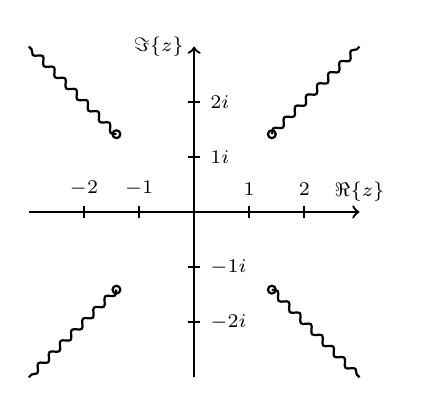
\begin{tikzpicture}[scale=0.7]
		    \begin{scope}[thick,font=\scriptsize]
		    % Axes:
		    % Are simply drawn using line with the `->` option to make them arrows:
		    % The main labels of the axes can be places using `node`s:
		    \draw [->] (-3,0) -- (3,0) node [above]  {$\Re\{z\}$};
		    \draw [->] (0,-3) -- (0,3) node [left] {$\Im\{z\}$};

		    % Points
    		\draw [decorate,decoration={snake,amplitude=.4mm,segment length=2mm}] (1.41,1.41) -- (3,3) node [draw=black, circle, fill=none, inner sep=1pt, pos=0] {};
    		\draw [decorate,decoration={snake,amplitude=.4mm,segment length=2mm}] (1.41,-1.41) -- (3,-3) node [draw=black, circle, fill=none, inner sep=1pt, pos=0] {};
    		\draw [decorate,decoration={snake,amplitude=.4mm,segment length=2mm}] (-1.41,1.41) -- (-3,3) node [draw=black, circle, fill=none, inner sep=1pt, pos=0] {};
    		\draw [decorate,decoration={snake,amplitude=.4mm,segment length=2mm}] (-1.41,-1.41) -- (-3,-3) node [draw=black, circle, fill=none, inner sep=1pt, pos=0] {};

		    % Axes labels:
		    % Are drawn using small lines and labeled with `node`s. The placement can be set using options
		    \iffalse% Single
		    % If you only want a single label per axis side:
		    \draw (1,-3pt) -- (1,3pt)   node [above] {$1$};
		    \draw (-1,-3pt) -- (-1,3pt) node [above] {$-1$};
		    \draw (-3pt,1) -- (3pt,1)   node [right] {$i$};
		    \draw (-3pt,-1) -- (3pt,-1) node [right] {$-i$};
		    \else% Multiple
		    % If you want labels at every unit step:
		    \foreach \n in {-2,...,-1,1,2,...,2}{%
		        \draw (\n,-3pt) -- (\n,3pt)   node [above] {$\n$};
		        \draw (-3pt,\n) -- (3pt,\n)   node [right] {$\n i$};
		    }
		    \fi
		    \end{scope}
		\end{tikzpicture}
		\caption{The complex numbers $z = 1 \pm i$ represented on an Argand diagram. }
	\end{subfigure}\hspace{1cm}%
	\begin{subfigure}{.4\linewidth}
		\centering
		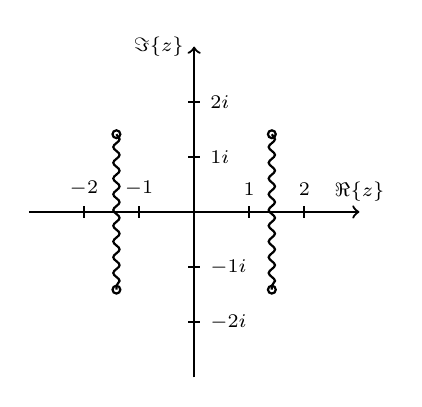
\begin{tikzpicture}[scale=0.7]
		    \begin{scope}[thick,font=\scriptsize]
		    % Axes:
		    % Are simply drawn using line with the `->` option to make them arrows:
		    % The main labels of the axes can be places using `node`s:
		    \draw [->] (-3,0) -- (3,0) node [above]  {$\Re\{z\}$};
		    \draw [->] (0,-3) -- (0,3) node [left] {$\Im\{z\}$};

		    % Points
    		\draw [decorate,decoration={snake,amplitude=.4mm,segment length=2mm}] (1.41,1.41) -- (1.41,-1.41) node [draw=black, circle, fill=none, inner sep=1pt, pos=1] {} node [draw=black, circle, fill=none, inner sep=1pt, pos=0] {};
    		\draw [decorate,decoration={snake,amplitude=.4mm,segment length=2mm}] (-1.41,1.41) -- (-1.41,-1.41) node [draw=black, circle, fill=none, inner sep=1pt, pos=1] {} node [draw=black, circle, fill=none, inner sep=1pt, pos=0] {};

		    % Axes labels:
		    % Are drawn using small lines and labeled with `node`s. The placement can be set using options
		    \iffalse% Single
		    % If you only want a single label per axis side:
		    \draw (1,-3pt) -- (1,3pt)   node [above] {$1$};
		    \draw (-1,-3pt) -- (-1,3pt) node [above] {$-1$};
		    \draw (-3pt,1) -- (3pt,1)   node [right] {$i$};
		    \draw (-3pt,-1) -- (3pt,-1) node [right] {$-i$};
		    \else% Multiple
		    % If you want labels at every unit step:
		    \foreach \n in {-2,...,-1,1,2,...,2}{%
		        \draw (\n,-3pt) -- (\n,3pt)   node [above] {$\n$};
		        \draw (-3pt,\n) -- (3pt,\n)   node [right] {$\n i$};
		    }
		    \fi
		    \end{scope}
		\end{tikzpicture}
		\caption{The complex numbers $z = 1 \pm i$ represented on an Argand diagram. }
	\end{subfigure}
	\caption{Two options for branch cuts for the function $f(z) = \sqrt{z^4 + 1}$.}
\end{figure}
\end{example}

\subsection{Logarithm and Exponential functions}

We define:

\[\exp{z} = \sum_{n=0}^\infty \frac{z^n}{n!} \]

By showing that $\exp{z_1}\exp{z_2} = \exp{z_1 + z_2}$, we can see $\exp{z}$ reduces to $\exp{x}$ for $\Im{z} = 0$, and so complex exponentials behave the same as real exponentials. For $a > 0$ we can write:

\[ a^z = \exp{z\ln{a}} \]

and so putting $a = e$ shows that $e^z$ and $\exp{z}$ are interchangeable.

We have already seen that logarithms require branch cuts. As a further demonstration, consider:

\begin{align*}
\ln{6} &= \ln{(-2)(-3)} \\
&\stackrel{*}{=} \ln{2e^{i\pi}} + \ln{3e^{i\pi}} \\
&= \ln{2} + i\pi + \ln{3} + i\pi \\
&= \ln{6} + 2i\pi
\end{align*}

At the starred step. we have simply expressed $-2$ and $-3$ in polar form. The extra factor fo $2i\pi$ represents us changing to the wrong branch. By introducing a branch cut from $0$ to $-\infty$, we restrict $\arg{z} \in [-\pi,\pi]$ and can then choose:

Instead using $-2 = 2e^{i\pi}$, $-3 = 3e^{-i\pi}$ giving $6 = (-2)(-3) = 6e^{0} = 6$.

\subsection{Trigonometric and Hyperbolic functions}

As we have considered the extension of the exponential function, the extension of trigonometric and hyperbolic functions follows trivially:

\begin{align*}
\cos{\theta} = \frac{e^{i\theta} + e^{-i\theta}}{2} &\longrightarrow \cos{z} = \frac{e^{iz} + e^{-iz}}{2}\\
\sin{\theta} = \frac{e^{i\theta} + e^{-i\theta}}{2} &\longrightarrow \sin{z} = \frac{e^{iz} - e^{-iz}}{2i}\\
\cosh{\theta} = \frac{e^{\theta} + e^{-\theta}}{2} &\longrightarrow \cosh{z} = \frac{e^{z} + e^{-z}}{2}\\
\sinh{\theta} = \frac{e^{\theta} + e^{-\theta}}{2} &\longrightarrow \sinh{z} = \frac{e^{z} - e^{-z}}{2}
\end{align*}

We see:

\begin{align}
\cos{z} &= \cosh{iz} \\
\sin{z} &= i\sinh{iz} \\
\cosh{z} &= \cos{iz} \\
\sinh{z} &= i\sin{iz}
\end{align}

This shows that the hyperbolic functions are periodic in the imaginary plane, in the same way that the trigonometric functions are periodic in the real plane. 

\section{Differentiation and Cauchy-Riemann Equations}

Recall $f'(x) = \lim_{h\to 0} \frac{f(x + h) - f(x)}{h}$. Before we can consider an extension of differentiation to the complex plane, we need to define a crucial property.

\subsection{Continuity}

A complex function $f(z)$ is called \emph{continuous} at $z$ when we have:

\[ \lim_{z\to z_0} f(z) = w \iff \forall \epsilon > 0 \exists \delta > 0 s.t. |z - z_0| < \delta \implies |f(z) - w] < \epsilon \]

This definition is the same in $\mathbb{C}$ as in $\mathbb{R}$, $\mathbb{R}^2$ etc. 

Note that for this definition to hold, we must have that $\lim_{z\to z_0} f(z)$ is path independent. 

We can now return to considering how to define differentiation.

\subsection{Differentiation}

Despite the fact that we can think of complex numbers as 2 dimensional vectors, we can't import vector derivatives into the complex plane. This becomes clear when we consider the domains and codomains of grad ($\grad$), div ($\div$), and curl ($\curl$):

\begin{align*}
\grad: \mathbb{R} &\longrightarrow \mathbb{R}^n \\
&\\
\div: \mathbb{R}^n &\longrightarrow \mathbb{R} \\
&\\
\curl: \mathbb{R}^3 &\longrightarrow \mathbb{R}^3 
\end{align*}

We clearly require a complex derivative $\vec{\nabla}_{\mathbb{C}}$ such that:

\[ \vec{\nabla}_{\mathbb{C}}: \mathbb{C} \longrightarrow \mathbb{C} \]

We will try to extend the real definition of the derivative to the complex plane. Consider:

\[ \vec{\nabla}_{\mathbb{C}} f = \frac{df}{dz} = \lim_{\delta\to 0} \frac{f(z+\delta) - f(z)}{\delta} \hspace{1in} \delta \in \mathbb{C}\]

In order to justify this definition, we will try some basic functions. 

Consider $f(z) = z$:

\begin{align*}
\frac{df}{dz} = \lim_{\delta\to 0} \frac{\cancel{z}+\delta - \cancel{z}}{\delta} = 1
\end{align*}

 \begin{align*}
\frac{df}{dz} &= \lim_{\delta\to 0} \frac{(z+\delta)^2 - z^2}{\delta} \\
&= \lim_{\delta\to 0} \frac{2\delta z - \delta^2}{\delta} \\
&= 2z
\end{align*}

Both of the above give the expected result. Now consider $f(z) = z^\star$:

\begin{align*}
\frac{df}{dz} &= \lim_{\delta\to 0} \frac{(z+\delta)^\star - z^2}{\delta} \\
&= \frac{\delta^\star}{\delta} 
\end{align*}

If $\delta = |\delta|e^{i\theta}$ then $\frac{\delta^\star}{\delta} = e^{-2i\theta}$, so the limit is not well-defined, hence $f(z) = z^\star$ is not differentiable. Finally, consider $f(z) = |z|^2 = z z^\star$:

\begin{align*}
\frac{df}{dz} &= \lim_{\delta\to 0} \frac{(z+\delta) (z+\delta)^\star - z z^\star}{\delta} \\
&= \frac{\delta z^\star + \delta^\star z + \delta \delta^\star}{\delta} \\
&= z^\star + z\frac{\delta^*}{\delta} + \mathcal{O}(\delta^2)
\end{align*}

So $f(z) = |z|^2$ is only differentiable at $z=0$, as $z\frac{\delta^*}{\delta}$ is only path-independent at $z=0$. This uncertainty in whether functions can be differentiated motivates us to introduce a new property of functions.

\subsection{Analytic Functions}

Firstly, we define a neighbourhood of $z\in \mathbb{C}$ as anopen set $U$ such that $z \in U$.

We can then say that $f: \mathbb{C} \leftarrow \mathbb{C}$ is analytic (or equivalently holomorphic) at $z_0 \in \mathbb{C}$ if $\exists$ a neighbourhood $U$ of $z_0$ on which $f$ is differentiable at all points in $U$.

Note that whilst $|z|^2$ is differentiable at $z = 0$, it is not analytic as it isn't differentiable in an arbitrarily small neighbourhood around $z=0$.

If a function $f$ is analytic on the neighbourhood $U = \mathbb{C}$, then it is called an \emph{entire} function.

\subsection{Cauchy-Riemann Equations}

We will now examine complex differentiation more rigorously. Consider $f(x + iy) = u(x,y) + iv(x,y)$. Then:

\begin{align*}
\frac{f(z) - f(z_0)}{z-z_0} &= \frac{u(x_0 + \delta x, y_0 + \delta y) -u(x_0, y_0)}{\delta x + i\delta y} + \frac{iv(x_0 + \delta x, y_0 + \delta y) - iv(x_0,y_0)}{\delta x + i\delta y} \\
&= \frac{\delta x \frac{\partial u}{\partial x} + \delta y \frac{\partial u}{\partial y}}{\delta x + i\delta y} + \frac{i \left(\delta x \frac{\partial v}{\partial x} + \delta y \frac{\partial v}{\partial y} \right)}{\delta x + i\delta y} + \mathcal{O}(\delta^2) \\
&= \frac{\delta x \left(\frac{\partial u}{\partial x} + i\frac{\partial v}{\partial x}\right) + i\delta y \left(-i\frac{\partial u}{\partial y} + \frac{\partial v}{\partial y}\right)}{\delta x _ i\delta y}
\end{align*}

In order to cancel the denominator and have $\lim_{z\to z_0} \frac{f(z) - f(z_0)}{z-z_0}$ exist, we require:

\[ \frac{\partial u}{\partial x} + i\frac{\partial v}{\partial x} = -i\frac{\partial u}{\partial y} + \frac{\partial v}{\partial y} \]

Equivalently:

\begin{align*}
\frac{\partial u}{\partial x} &= \frac{\partial v}{\partial y} \\
\frac{\partial v}{\partial x} &= -\frac{\partial u}{\partial y}
\end{align*}

Once again, consider: 

\[ f(z) = z^2 = (x + iy)^2 = x^2 - y^2 + 2ixy \]

So:

\begin{align*}
u &= x^2 - y^2 :  & \frac{\partial u}{\partial x} = 2x \hspace{1cm} & \frac{\partial u}{\partial y} = -2y \\
v &= 2xy : & \frac{\partial v}{\partial x} = 2y \hspace{1cm} & \frac{\partial v}{\partial y} = 2x 
\end{align*}

So we have $\frac{\partial u}{\partial x} = \frac{\partial v}{\partial y}$, $\frac{\partial v}{\partial x} = -\frac{\partial u}{\partial y}$ so $f(z) = z^2$ is \emph{entire}, as we didn't place any restrictions on $z_0$ at the start of the process. 

Note that these equalities imply $u$ obeys a Laplace equation:

\begin{align*}
\frac{\partial^2 u}{\partial x^2} &= \frac{\partial}{\partial x}\frac{\partial u}{\partial x} = \frac{\partial}{\partial x} \frac{\partial v}{\partial y} = \frac{\partial^2 v}{\partial x \partial y} = \frac{\partial}{\partial y}\frac{\partial v}{\partial x} = -\frac{\partial}{\partial y}\frac{\partial u}{\partial y} = -\frac{\partial^2 u}{\partial y^2} \\
&\implies \frac{\partial^2 u}{\partial x^2} + \frac{\partial^2 u}{\partial y^2} = 0
\end{align*}

Suppose we consider $z$ and $z^\star$ to be independent functions. We can write:

\[ x = \frac{z + z^\star}{2}, \; y = \frac{z - z^\star}{2i} \]

Then 

\begin{align*} 
\frac{\partial}{\partial z^\star} &= \frac{\partial x}{\partial z^\star}\frac{\partial}{\partial x} + \frac{\partial y}{\partial z^\star}\frac{\partial}{\partial y}\\
&= \frac{1}{2}\left(\frac{\partial}{\partial x} + i\frac{\partial}{\partial y} \right)
\end{align*}

Giving:

\[ \frac{\partial f}{\partial z^\star} = \frac{1}{2}\left(\frac{\partial u}{\partial x} + i\frac{\partial u}{\partial y} + i\frac{\partial v}{\partial x} - \frac{\partial v}{\partial y}\right) = 0 \]

if and only if the Cauchy-Riemann equations hold. Hence $\frac{\partial f}{\partial z^\star} = 0$ forms a compact test for analyticity. 
\end{document}